\section{OD Energy Scale} \label{sec:od_energy_scale}
\par
After construction and filling of the OD, the SPE for each PMT was checked using the OD optical calibration system (OCS) \cite{lz_ocs_system_ref}.
A detailed description of the PMT monitoring during commissioning and SR1 can be found in the works of E. Fraser \cite{ewanfraser_thesis_ref}. 
During this period, an energy calibration of the OD was also performed.
Again, details of the methodology are described in \cite{ewanfraser_thesis_ref} but summarised below, as the result is used throughout this chapter to evaluate the requirements described in \autoref{sec:simulated_od_requirements}.
\par
Of the sources mentioned in \autoref{sec:lz_detector_chapter} 7 $\gamma$ sources were used.
Each were lowered into the CSD's to the 700mm level (see \autoref{fig:CSD1_Geometry}).
The sources used are summarised in \autoref{tab:od_energy_calibration_sources}.

\begin{table}[!htbp]%
    \centering
    \begin{tabular}{c|c|c}
        Source      & Specific observable         &  $\gamma$ energy (keV) \\ \hline
        ${}^{57}Co$ & direct $\gamma$             & 122                        \\
        ${}^{22}Na$ & positron annihilation       & 511               \\
        ${}^{54}Mn$ & direct $\gamma$             & 835                        \\
        ${}^{22}Na$ & direct $\gamma$             & 1275               \\
        ${}^{252}Cf$ & neutron capture on H       & 2223            \\
        ${}^{228}Th$ & ${}^{208}Tl$ $\beta-$decay & 2615            \\
        ${}^{252}Cf$ & neutron capture on Gd      & 8000            
        
    \end{tabular}
    \caption{Calibration sources used to determine the OD energy scale.}
    \label{tab:od_energy_calibration_sources}
\end{table}

\par
As discussed in \autoref{sec:od_physics}, there is a non-linear energy response in the scintillator, and therefore a non-linear energy scale below 300keV.
The empirical formula for the non-linear energy response of the scintillator from DayaBay \cite{dayabay_antineutrino_oscillation_ref, ls_nonlinear_energy_response_ref}, shown in \autoref{eq:ls_light_response}, was used to fit to these points.
\begin{equation}
    \frac{E_{vis}}{E_{true}} = \frac{p_0  + p_3 \times E_{true}}{1 + p_1 \times e^{p_2 \times E_{true}}}
    \label{eq:ls_light_response}
\end{equation}
The fit and the translation from photons detected to energy are shown in \autoref{fig:od_energy_scale}.

\begin{figure}[]
    \centering
   \begin{tikzpicture}
    \begin{groupplot}[%view={0}{90},
    group style = {group size = 1 by 2,vertical sep=0.5cm},
                   width=0.98\textwidth]
    \nextgroupplot[
            ylabel=LS energy response ($\frac{E_{vis}}{E_{true}}$),
            %xlabel=,
            xticklabels={,,}
            height=10cm, width=\textwidth,
            xmin=0, xmax=10,
            grid=major,
            ]
            %\addplot[black, smooth, domain=0:10] 
                    %{(0.00535 + 0.0286*x) / (1-0.9918*exp(-0.03018*x))};
                    %{((0.001894 + 0.03614*x) / (1-1*exp(-0.001453*x)))};
            \addplot[black, smooth]
                table[x=Energy,y=Value]
                {Data/OD_Energy_Scale/emperical_fit.dat};
                    
            \addplot[only marks,
                 error bars/.cd,
                 y dir=both, y explicit, error bar style={color=black}] table[x=Energy,y=light_response, y error=light_response_Error] {Data/OD_Energy_Scale/phd_energy.dat};

    \nextgroupplot[
            ylabel=N. photons detected,
            xlabel=Energy (MeV),
            height=6cm, width=\textwidth,
            xmin=0, xmax=10,
            ymin=0, 
            grid=major,
            ]
            \addplot[only marks,
                 error bars/.cd,
                 y dir=both, y explicit, error bar style={color=black}] table[x=Energy,y=pulseArea, y error=pulseArea_Error] {Data/OD_Energy_Scale/phd_energy.dat};
            \addplot[black, smooth, domain=0:10] 
                    {-33.98 + 0.2425*x*1000};
            
  \end{groupplot}
    \end{tikzpicture}
    \caption{OD Energy Scale and the relation between observed number of photons and the energy deposited. Analysis by E. Fraser \cite{ewanfraser_thesis_ref}.}
    \label{fig:od_energy_scale}
\end{figure}

%    \nextgroupplot[
%            ylabel=N. photons detected,
%            xlabel=Energy (MeV),
%            height=6cm, width=\textwidth,
%            xmin=0, xmax=10,
%            ymin=0, 
%            grid=major,
%            ]
%            \addplot[black]
%                    table [x=Energy,y=Value]
%                    {Data/OD_Energy_Scale/phd.dat};

\par
A comparison to other LAB-based experiments is provided in \autoref{tab:od_phe_per_mev_comparison}.

\begin{table}[!htbp]%
    \centering
    \begin{tabular}{c|c}
        Detector & phe/MeV \\ \hline
        RENO     & 150 \cite{reno_phe_per_mev_ref} \\
        Borexino & 438 \cite{pablo_mosteiro_thesis_ref} \\
        Daya Bay & 162 \cite{dayabay_phe_per_mev_ref} \\
        Kamland  & 200 \cite{kamland_phe_per_mev_ref} \\
        SNO+     & 300 \cite{snoplus_phe_per_mev_ref} \\
        LZ       & 230 
    \end{tabular}
    \caption{LZ OD photons detected per electron equivalent MeV deposited compared to other large LAB experiments.}
    \label{tab:od_phe_per_mev_comparison}
\end{table}

\subsection{Fit Uncertainty}
\par
Perhaps the largest drawback in the energy calibration is that only a single location was used, in Z.
Therefore the variation in light collection efficiency in the OD could not be taken into account, see \autoref{fig:od_lce}.
This is tested in the following Section and shown in be insignificant.


\subsection{PMT Noise}
\par
Observations of waveforms showed that there was a grounding issue, which occasionally caused high energy pulses with large PMT multiplicities.
An waveform of this is shown in \autoref{fig:noise_od_waveform} where during the noise period no physical OD event can be made out from the noise.
Included as well is an example of OD data during a quiet period of data taking showing a rate as expected.

\begin{figure}[]
\begin{subfigure}{\textwidth}
  \centering
  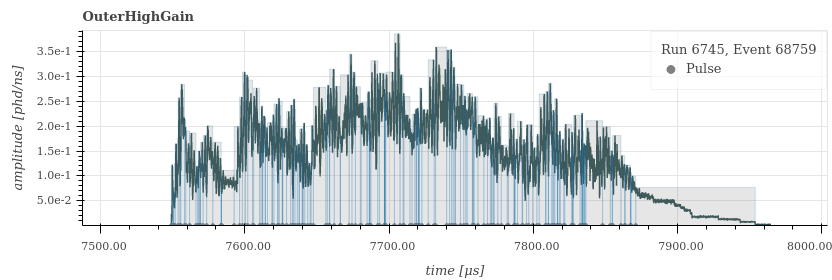
\includegraphics[width=\linewidth]{Figures/OD_Backgrounds/noise_pulse.png}
  \caption{High noise period.}
  \label{fig:noise_od_waveform}
  \end{subfigure}
  \begin{subfigure}{\textwidth}
  \centering
  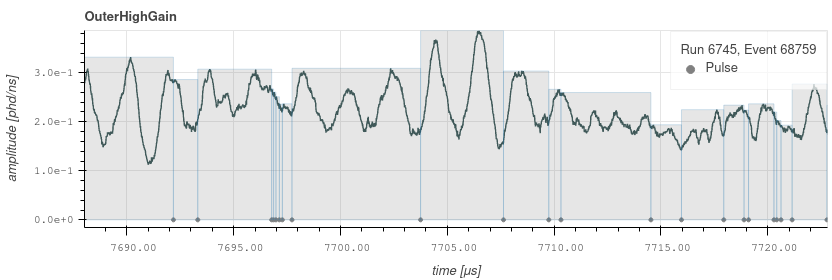
\includegraphics[width=\linewidth]{Figures/OD_Backgrounds/noise_pulse_zoomed.png}
  \caption{High noise period zoomed}
  \label{fig:noise_od_waveform_zoomed}
  \end{subfigure}
  \begin{subfigure}{\textwidth}
  \centering
  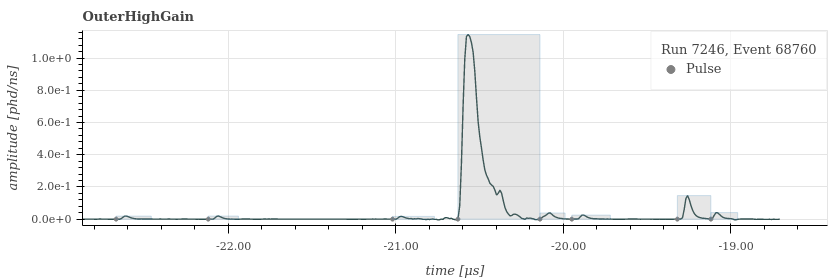
\includegraphics[width=\linewidth]{Figures/OD_Backgrounds/regular_pulse.png}
  \caption{Regular pulses}
  \label{fig:regular_od_waveform}
  \end{subfigure}
\caption{OD summed waveforms showing a noisy period of data and a regular period.}
\label{fig:od_noise_cut_waveforms}
\end{figure}


\begin{figure}[]%
\centering
\begin{tikzpicture}
\centering
  \begin{axis}[%point meta max=150,
    %point meta min=0.0,
    height=10cm, width=10cm,
    view={0}{90},
    ylabel={Pulse Amplitude/Pulse Area},
    xlabel={Pulse Area (phd)},
    xmin=0, ymin=0,
    colorbar,
    colorbar style={ylabel={Count (log$_{10}$}),},
    ]
    \addplot3[
      surf,
      shader=flat corner,
	  mesh/cols=22,
	  mesh/ordering=rowwise,
	  point meta = {z<0.1 ? nan : z}
    ] file {Data/OD_Energy_Scale/noise_cut_2d_low_2.dat};
    
    \addplot3[
      surf,
      shader=flat corner,
	  mesh/cols=30,
	  mesh/ordering=rowwise,
	  point meta = {z<0.1 ? nan : z}
    ] file {Data/OD_Energy_Scale/noise_cut_2d_high_2.dat};
\end{axis}
\end{tikzpicture}
\caption{Representative pulses seen in the OD during SR1.
         No pulse selection has been applied.
         Real events are in the distribution around 0.01 height/area.}
\label{fig:od_noise_cut}
\end{figure}

\par
In order to counteract this, a noise cut was developed to remove this based upon the pulse shape, requiring that a large portion of the pulse integral be within 100ns of the pulse starting.
Combined with a requirement of a PMT multiplicity of 5, the background noise and PMT dark rates and after pulsing were removed.
This combined selection is used throughout this chapter being referred to as the "noise cut".

\begin{figure}
    \centering
    
\includegraphics[width=0.5\textwidth]{Figures/Placeholder.png}
    \caption{Cut application}
    \label{fig:od_noise_cut}
\end{figure}